
\section{用\trEffectiveCartierDivisor{}{}\trSlicing{}、\trRegularSequence{}与\trRegularEmbedding{}}

我们现在引入\trRegularEmbedding{}（regular embedding）——局部闭嵌入中重要的一类。从\trRegular\trScheme{}到\trRegular\trScheme{}之内的局部闭嵌入，便是\trRegularEmbedding{}的一个重要例子（\mbox{练习~13.2.M}(b)）。有效卡蒂耶除子（effective Cartier divisor）——基本上就是余维数 $1$ 的情形——日后也将被一再证明有用；「反复用有效卡蒂耶除子\trSlicing{}」为许多论证提供了归纳步骤。（今后在许多语境下，当我们说\textbf{\trSlicing{}}（slicing）时，指的都是用有效卡蒂耶除子作\trSlicing{}。）

\textbf{9.5.1.\ \trLocallyPrincipal{}闭子概形，与有效卡蒂耶除子。}\quad 一个\trClosedSubscheme{}称为\textbf{\trLocallyPrincipal{}}（locally principal）的，若在足够细的一个\trOpenCover{}的每个\trOpenSet{}上，它都由单个方程切出（也就是说，由一个\trPrincipalIdeal{}切出——术语正由此得名）。更确切地说，\trLocallyPrincipal{}闭子概形是这样的\trClosedSubscheme{} $\pi\colon X\hookrightarrow Y$：存在 $Y$ 的一个\trOpenCover{} $\{U_i\}$，使得对每个 $i$，$\pi^{-1}(U_i)\hookrightarrow U_i$ 都\trIsomorphic{}于某个形如 $V(s_i)\hookrightarrow U_i$ 的\trClosedSubscheme，其中 $s_i\in\Gamma(U_i,\OO_Y)$。（这个\trOpenCover{}显然可以取成由\trAffine\trOpenSubset{}组成的。）

例如，$\mathbb{P}^n_k$ 中的超曲面（定义~9.3.2）就是\trLocallyPrincipal{}的：$n+1$ 个变元之间的每个齐次多项式都定义了 $\mathbb{P}^n_A$ 的一个\trLocallyPrincipal{}闭子概形。（\trhWarning：与「\trLocallyPrincipal{}性」不同，「主性」并不是一个仿射局部条件；见 \S19.11.10！此外，射影超曲面的例子（\S9.3.1）表明：\trLocallyPrincipal{}闭子概形未必由一个整体有定义的函数切出。最后，很遗憾，在 \S15.4.8 中我们会以另一种意思使用「\trLocallyPrincipal{}」这个说法。）

若\trIdealSheaf{}在每一点附近都由一个\trNonZerodivisor{}函数局部生成，我们就称这个闭子概形为一个有效卡蒂耶除子。更确切地说：若 $\pi\colon X\to Y$ 是一个\trClosedEmbedding，且存在由\trAffine\trOpenSubset{} $\Spec A_i\subset Y$ 组成的 $Y$ 的\trCover，并存在\trNonZerodivisor{} $t_i\in A_i$ 使 $V(t_i)=X|_{\Spec A_i}$（在概形论的意义下——也就是说，$X$ 在 $\Spec A_i$ 上的\trIdealSheaf{}由 $t_i$ 生成），那么我们就说 $X$ 是 $Y$ 上的一个\textbf{\trEffectiveCartierDivisor{}{}}。（这个说法的来历我们不作解释，因为它与这里的视角无关。）当我们意指「限制到一个有效卡蒂耶除子上」时，常会用「\textbf{用}一个有效卡蒂耶除子\textbf{\trSlicing{}}」（slicing by an effective Cartier divisor）这个形象的说法。

有效卡蒂耶除子这个观念是核心性的；\trLocallyPrincipal{}闭子概形这个观念则远非如此。

\textbf{9.5.A.（练习）}\quad 设 $t\in A$ 是一个\trNonZerodivisor。证明：对每个\trPrimeIdeal{} $p$，$t$ 在 $A_p$ 中都是\trNonZerodivisor。

\textbf{9.5.2.}\ \emph{\trhCaveat{}。}\quad 若 $D$ 是\trAffineScheme{} $\Spec A$ 上的一个有效卡蒂耶除子，则未必存在 $t\in A$ 使 $D=V(t)$（见\mbox{练习~15.5.I}——\S19.11.10 给出了另一种风味的例子）。换言之，「闭子概形是有效卡蒂耶除子」这一条件可以在\emph{某个}仿射覆盖上得到验证，却不能在\emph{任意}仿射覆盖上检验——它并不是这种显而易见意义上的仿射局部条件。

\textbf{9.5.B.（练习）}\quad 设 $X$ 是一个局部\trNoetherian{}概形。若 $t\in\Gamma(X,\OO_X)$ 是 $X$ 上的一个函数，证明：$t$（或更确切地说，闭子概形 $V(t)$）是一个有效卡蒂耶除子，当且仅当它在 $X$ 的任何\trAssociatedPoint{}上都不消失。证明：$X$ 的一个\trLocallyPrincipal{}闭子概形是有效卡蒂耶除子，当且仅当它不包含 $X$ 的任何\trAssociatedPoint。

\textbf{9.5.C.（练习）}\quad 设 $V(t)=V(t')\hookrightarrow\Spec A$ 是一个有效卡蒂耶除子，其中 $t$ 与 $t'$ 都是 $A$ 中的\trNonZerodivisor。证明：$t$ 是 $t'$ 的可逆函数倍。

有效卡蒂耶除子的想法把我们引向\trRegularSequence（regular sequence）的观念。（我们将在\mbox{练习~9.5.H}中完成闭环：届时我们将把任何合理概形上的有效卡蒂耶除子解读为余维数 $1$ 的\trRegularEmbedding{}。）

\textbf{9.5.3.\ \trRegularSequence{}。}\quad 「正则序列」这个观念——如同其他许多观念一样——归功于\trSerre{}[Se2]。正则序列的定义，是下述几何想法的代数版本：局部地，我们取一个有效卡蒂耶除子（一个\trNonZerodivisor）；然后再取其上的一个有效卡蒂耶除子；然后再取其上的一个有效卡蒂耶除子；如此进行，做有限多次。这里需要一点小心；比如说，我们可能希望这件事与所加方程的次序无关，而只有在我们把这话说对的时候，这才是真的。

我们对环 $A$ 给出\trRegularSequence{}的定义，并对 $A$-\trModule{} $M$ 作更一般的叙述。

\textbf{9.5.4.}\ \emph{\trhDefinition{}。}\quad 若 $M$ 是一个 $A$-\trModule，则 $A$ 中元素组成的序列 $x_1,\dots,x_r$ 称为一条\textbf{$M$-\trRegularSequence}（$M$-regular sequence；或\textbf{对 $M$ 的\trRegularSequence}，regular sequence for $M$），若下述两个条件得到满足。
\begin{enumerate}[label=(\roman*)]
\item 对每个 $i$，$x_i$ 都不是 $M/(x_1,\dots,x_{i-1})M$ 的\trZerodivisor。（$i=1$ 的情形应解读为：「$x_1$ 不是 $M$ 的\trZerodivisor」。回想：\trZerodivisor{}定义于\cref{ex:when-localization-is-injective}。）
\item 我们有真包含 $(x_1,\dots,x_r)M\subsetneq M$。
\end{enumerate}

在我们最关心的情形 $M=A$ 中，这应当被看作「\trCompleteIntersection」（complete intersection）的一个合理近似；而且事实上我们就将把它当作定义来使用（\S9.5.7）。

对\trRegularSequence{} $x_1,\dots,x_r\in A$，我们称 $r$ 为\textbf{\trRegularSequence{}的\trLength}。一条 $A$-\trRegularSequence{}就径直称为\textbf{\trRegularSequence}。

\textbf{9.5.D.（练习）}\quad 若 $M$ 是一个 $A$-\trModule，证明：一条 $M$-\trRegularSequence{}在任何局部化之后，仍满足\trRegularSequence{}的定义~9.5.4 中的条件 (i)。（等你懂得了何为\trFlatness{}之后，你将会看到：你的论证恰恰表明条件 (i) 在任何平坦\trBaseChange{}下保持。）

\textbf{9.5.E.（练习）}\quad 若 $x,y$ 是一条 $M$-\trRegularSequence，证明：$x^N,y$ 也是一条 $M$-\trRegularSequence。提示：困难的部分在于证明 $y$ 不是 $M/(x^N M)$ 的\trZerodivisor。请对 $N$ 作归纳来证明这一点。若 $y$ 是 $M/(x^N M)$ 的\trZerodivisor，则对某个 $m\in M\setminus x^N M$ 有 $ym\equiv 0\pmod{x^N}$。于是 $ym=x^N k$，其中 $k\in M$。利用「$x,y$ 是一条\trRegularSequence」这一事实，证明 $m$ 是 $x$ 的倍数。（你的论证将可以轻易推广，从而更一般地证明：若 $x_1,\dots,x_n$ 是一条\trRegularSequence，而 $a_1,\dots,a_n\in\mathbb{Z}^+$，则 $x_1^{a_1},\dots,x_n^{a_n}$ 是一条\trRegularSequence。）

\textbf{9.5.5.}\ \emph{序列的正则性依赖于其次序。}\quad 我们现在给出一个例子（[E, Example 17.3]），表明\trRegularSequence{}的次序是有关系的。设 $A=k[x,y,z]/(x-1)z$，于是 $X=\Spec A$ 是平面 $z=0$ 与平面 $x=1$ 之并——$X$\trReduced，且有两个\trIrreducibleComponent（见图~\ref{fig:regular-sequence-order}）。你可以轻而易举地核验：$x$ 是 $A$ 的\trNonZerodivisor（$x=0$ 错过 $X$ 的一个\trIrreducibleComponent，而在另一个上也不完全消失），并且相应的有效卡蒂耶除子 $X'=\Spec k[x,y,z]/(x,z)$（在 $X$ 上）是\trIntegral{}的。于是 $(x-1)y$ 给出 $X'$ 上的一个有效卡蒂耶除子（它在 $X'$ 上不完全消失），故 $x,(x-1)y$ 是 $A$ 的一条正则序列。然而，$(x-1)y$ 并\emph{不}是 $A$ 的\trNonZerodivisor，因为它\emph{确实}在两个\trIrreducibleComponent{}之一上完全消失。于是 $(x-1)y,x$ 就\emph{不}是正则序列。重排\trRegularSequence{} $x,(x-1)y$ 会毁掉正则性，其缘由是清楚的：存在一个\trLocus，在其上 $(x-1)y$ 并非有效卡蒂耶；但若我们先强加 $x=0$，它就不见了。这里的问题是一种「非局部性」——在「$x=y=z=0$ 附近」根本没有问题。这或许可以让我们预感到：在（\trNoetherian{}的）局部情势下，这个问题会消失。我们现在把这件事说精确。

\textbf{9.5.6.\ \trhTheorem{}。}\ ——\ \emph{设 $(A,\mathfrak{m})$ 是一个\trNoetherian{}\trLocalRing，$M$ 是一个有限生成的 $A$-\trModule。那么含于 $\mathfrak{m}$ 中的任何 $M$-\trRegularSequence{} $(x_1,\dots,x_r)$ 在任何重排之下仍是\trRegularSequence。}

（在 [Di] 中，\trDieudonne{}给出了一个占半页的例子，表明\trNoetherian{}假设在定理~9.5.6 中是必需的。此外，在\mbox{练习~24.6.C}中，当 $A$ 包含一个域时，我们给出了一个不同的、多少要简单些的证明。）

在证明定理~9.5.6 之前（证明见于\mbox{练习~9.5.F}），我们先证第一个非平凡情形，即 $r=2$ 的情形。这段讨论暗地里是 Koszul 复形（Koszul complex）的一个婴孩情形（\S24.4.1 将简要提到这个复形）。

\begin{figure}[htbp]
\centering
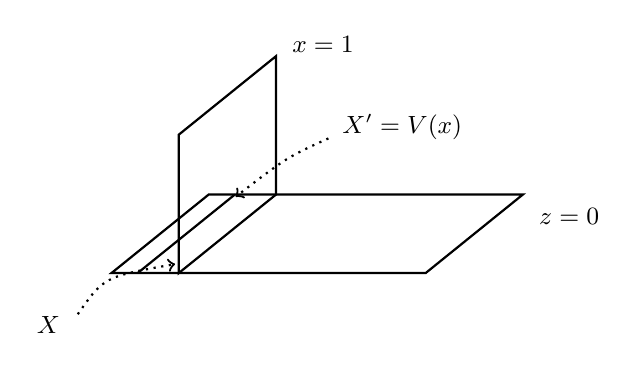
\begin{tikzpicture}[scale=0.95,line width=0.8pt,every node/.style={font=\small}]
  \draw (0,0) -- (4.2,0) -- (5.5,1.05) -- (1.3,1.05) -- cycle;
  \draw (0.35,0) -- (1.65,1.05);
  \draw (0.9,0) -- (2.2,1.05) -- (2.2,2.9) -- (0.9,1.85) -- cycle;
  \node[anchor=west] at (2.28,3.05) {$x=1$};
  \node[anchor=west] at (5.58,0.75) {$z=0$};
  \node[anchor=west] at (2.95,1.95) {$X' = V(x)$};
  \draw[dotted,->] (2.9,1.8) .. controls (2.35,1.55) .. (1.66,1.02);
  \node[anchor=east] at (-0.55,-0.7) {$X$};
  \draw[dotted,->] (-0.45,-0.55) .. controls (-0.1,-0.05) .. (0.85,0.12);
\end{tikzpicture}
\caption{\trRegularSequence{}中次序有关系（在「非局部」的情势下），理由毫不令人惊讶。（依原书手绘图重绘。）}\label{fig:regular-sequence-order}
\end{figure}

设 $\mathfrak{m}$ 中的元素 $x$ 与 $y$ 组成一条 $M$-\trRegularSequence。翻译过来就是：$x\in\mathfrak{m}$ 在 $M$ 上是\trNonZerodivisor，而 $y\in\mathfrak{m}$ 在 $M/xM$ 上是\trNonZerodivisor。

考察\trDoubleComplex
\begin{equation*}\tag{9.5.6.1}\label{eq:double-complex-regular-sequence}
\begin{tikzcd}[row sep=3em, column sep=4.2em]
M \ar[r, "\times(-x)"] & M \\
M \ar[u, "\times y"] \ar[r, "\times x"] & M, \ar[u, "\times y"]
\end{tikzcd}
\end{equation*}
其中左下角被认为处于位置 $(0,0)$。（上一行出现负号的唯一理由，是我们在 \S1.6.1 中偏爱反交换方块而非交换方块的任意口味；但它实在无关紧要。）

我们用一条（简单的）\trSpectralSequence{}来计算\trTotalComplex{}的\trCohomology，从右行定向开始。（在这里动用谱序列——正如在我们其他许多应用中那样——实属大材小用；我们这么做，部分是为了练一练这台机器。）在第一\trPage，我们有
\begin{equation*}\tag{9.5.6.2}\label{eq:regular-sequence-first-page}
\begin{tikzcd}[row sep=3.2em, column sep=4.5em]
\ker\bigl(M\mathrel{\xrightarrow{\ \times x\ }}M\bigr) & M/xM \\
\ker\bigl(M\mathrel{\xrightarrow{\ \times x\ }}M\bigr) \ar[u, "\times y"] & M/xM. \ar[u, "\times y"]
\end{tikzcd}
\end{equation*}
第一列中的诸 $\ker\bigl(M\mathrel{\xrightarrow{\ \times x\ }}M\bigr)$ 都是 $0$，因为 $x$ 在 $M$ 上是\trNonZerodivisor。在竖直方向取\trHomology{}以得到第二\trPage，我们发现
\begin{equation*}\tag{9.5.6.3}\label{eq:regular-sequence-second-page}
\begin{array}{c@{\qquad}c}
0 & M/(x,y)M\\[0.8em]
0 & 0,
\end{array}
\end{equation*}
这里用到了 $y$ 在 $M/xM$ 上是\trNonZerodivisor{}这一事实。该\trSpectralSequence{}显然在此处\trConverge。于是，原来的\trDoubleComplex{} \eqref{eq:double-complex-regular-sequence} 只在次数 $2$ 处有非零\trCohomology，且在该处\trCohomology{}为 $M/(x,y)M$。

现在我们改用上行定向对 \eqref{eq:double-complex-regular-sequence} 跑一遍\trSpectralSequence。这条\trSpectralSequence{}的第一\trPage{}为：
\[
\begin{tikzcd}[row sep=4.6em, column sep=5.5em]
M/yM \ar[r, "\times(-x)"] & M/yM \\
\ker\bigl(M\mathrel{\xrightarrow{\ \times y\ }}M\bigr) \ar[r, "\times x"] & \ker\bigl(M\mathrel{\xrightarrow{\ \times y\ }}M\bigr).
\end{tikzcd}
\]
该\trSpectralSequence{}在下一步之后必定\trConverge{}到 \eqref{eq:regular-sequence-second-page}。从上一行可以看出：乘 $x$ 在 $M/yM$ 上必定是单射，故 $x$ 在 $M/yM$ 上是\trNonZerodivisor。从下一行可以看出：乘 $x$ 给出 $\ker\bigl(M\mathrel{\xrightarrow{\ \times y\ }}M\bigr)$ 与自身之间的一个\trIsomorphism。由于 $x\in\mathfrak{m}$，据\trNakayama{}引理版本~2（引理~8.2.9），这就蕴含 $\ker\bigl(M\mathrel{\xrightarrow{\ \times y\ }}M\bigr)=0$，故 $y$ 在 $M$ 上是\trNonZerodivisor。于是我们便证明了：$y,x$ 构成 $M$ 上的一条\trRegularSequence——这正是定理~9.5.6 的 $r=2$ 情形。

\textbf{9.5.F.（容易练习）}\quad 证明定理~9.5.6。（提示：先证只交换两个相邻 $x_i$ 的那种重排，用刚才讨论的 $r=2$ 情形。）\trNoetherian{}假设都是在哪些地方被用到的？

\textbf{9.5.7.\ \trRegularEmbedding{}。}\quad 设 $\pi\colon X\hookrightarrow Y$ 是一个局部闭嵌入。我们说 $\pi$ \textbf{在点 $p\in X$ 处是（余维数 $r$ 的）\trRegularEmbedding{}}（regular embedding (of codimension $r$) at a point），若在\trLocalRing{} $\OO_{Y,p}$ 中，$X$ 的\trIdeal{}由一条（长度为 $r$ 的）\trRegularSequence{}生成。我们说 $\pi$ 是一个\textbf{（余维数 $r$ 的）\trRegularEmbedding{}}，若它在所有 $p\in X$ 处都是（余维数 $r$ 的）\trRegularEmbedding{}。（\trRegularEmbedding{}的另一个合理的名字本来可以是「局部完全相交」（local complete intersection）。不幸的是，「局部完全相交态射」（local complete intersection morphism），或「lci 态射」（lci morphism），已被用来指另一个相关的观念；见 [Stacks, tag 068E]。）

我们的术语用到了「余维数」这个词，而我们尚未把这个词单独当作一个词来定义。使用这个词的理由，在你见到\trKrull{}主理想定理~12.3.3 与\trKrull{}高度定理~12.3.10 之后，会变得更清楚。

\textbf{9.5.G.（练习：局部闭嵌入为\trRegularEmbedding{}这一条件是开的）}\quad 证明：若局部\trNoetherian{}概形之间的局部闭嵌入 $\pi\colon X\hookrightarrow Y$ 在 $p$ 处是\trRegularEmbedding{}，则它在 $X$ 中 $p$ 的某个\trOpen\trNeighborhood{}上都是\trRegularEmbedding{}。提示：先化归到 $\pi$ 是闭嵌入的情形，再化归到 $Y$（从而 $X$）仿射的情形——比如说 $Y=\Spec B$、$X=\Spec B/I$、$p=[p]$——并且存在 $f_1,\dots,f_r$，使得在 $\OO_{Y,p}$ 中诸 $f_i$ 的像组成一条生成 $I_p$ 的正则序列。我们希望证明：在「$p$ 的某个\trOpen\trNeighborhood{}中」有 $(f_1,\dots,f_r)=I$。请证明下述代数事实：若 $I$ 与 $J$ 是\trNoetherian{}环 $A$ 的两个\trIdeal，而 $p\subset A$ 是满足 $I_p=J_p$ 的一个\trPrimeIdeal，则存在 $a\in A\setminus p$ 使得在 $A_a$ 中 $I_a=J_a$。为证此，请先证明只需考虑 $I\subset J$ 这一特殊情形——做法是改考虑 $I\cap J$ 与 $J$。为证这一特殊情形，令 $K=J/I$（一个有限生成的\trModule），并证明：若 $K_p=0$，则对某个 $a\in A\setminus p$ 有 $K_a=0$。

于是，若 $X$ 在一个域上\trLocally\trFiniteType（例如是一个\trVariety），则要检验一个闭嵌入 $\pi$ 是不是\trRegularEmbedding{}，只需在 $X$ 的诸\trClosedPoint{}处检验就够了（\mbox{练习~5.3.F}）。

\mbox{练习~13.1.F}(b) 将证明：并非所有闭嵌入都是\trRegularEmbedding{}。

\textbf{9.5.H.（练习）}\quad 证明：局部\trNoetherian{}概形的闭嵌入 $X\hookrightarrow Y$ 是余维数 $1$ 的\trRegularEmbedding{}，当且仅当 $X$ 是 $Y$ 上的一个有效卡蒂耶除子。不重要的注记：\trNoetherian{}假设可以换成要求 $\OO_Y$ \trCoh，论证本质上照旧。有意思的是：「有效卡蒂耶除子」永远蕴含「余维数 $1$ 的\trRegularEmbedding{}」，但逆向的论证却需要\trNoetherian（或类似）的假设。（逆向命题的反例见 [MO129242]。）

\textbf{9.5.8.}\ \emph{\trhDefinition{}。}\quad 概形 $Y$ 中的一个\textbf{余维数 $r$ 完全相交}（codimension $r$ complete intersection）是一个闭子概形 $X$：它可以写成 $r$ 个有效卡蒂耶除子 $D_1,\dots,D_r$ 的\trSchemeTheoretic{}交，使得在每一点 $p\in X$ 处，与 $D_1,\dots,D_r$ 相应的方程都组成一条正则序列。\textbf{\trCompleteIntersection{}}这个说法意指「对某个 $r$ 的余维数 $r$ 完全相交」。
